In this chapter, we present an application of knowledge-guided reasoning. We
build a neural semantic parser for question answering over a challenging
dataset, and show how the model benefits from additional knowledge.  In
particular, we will discuss how sequence-to-sequence models, which have been
shown to work very well for modeling sequences in language, should be adapted to
work for semantic parsing.  Recent work has shown that such models can be used
for semantic parsing by encoding the question then predicting each token of the
logical form in sequence~\citep{jia2016,dong2016}.  These approaches, while
effective, have two major limitations.  First, they treat the logical form as an
unstructured sequence, thereby ignoring type constraints on well-formed
programs.  Second, they do not deal with entity linking, which is a critical
sub-problem of semantic parsing~\citep{yih2015stagg}.  To address these issues,
we modify the encoder-decoder model to:
\begin{enumerate}
	\item Constrain the decoder to only produce syntactically and semantically
		valid logical forms
	\item Incorporate context-awareness into the encoder, and entity linking
		into the decoder, to effectively score previously
		unseen entities by linking them to tokens in the
		utterance, and jointly train these entity embedding anr linking
		modules from QA supervision.
\end{enumerate}
We assume weak supervision, and train using Static MML (see Section~\ref{sec:mml})
on pairs of questions and approximate sets of logical forms that yield the correct answer,
but are not necessarily true translations of the questions. However, the two main
contributions of this chapter are also applicable to the fully supervised setup.
We now describe in detail the problems we solve in this chapter.

\section{Need for Grammar Constraints}
Sequence-to-sequence models~\citep{sutskever:14}, have been successfully used for Machine
Translation~\citep[among many
others]{sutskever:14,cho2014learning,bahdanau2014neural,wiseman2016sequence,artetxe2017unsupervised},
Summarization~\citep[among others]{Nallapati2016AbstractiveTS,Paulus2017ADR},
and other kinds of text generation tasks like dialogue
generation~\citep[for one]{li2017adversarial} and generation with style
control~\citep[for one]{ficler2017controlling}. In all these cases, and also most
other cases where encoder-decoder models are used for transducing language
inputs, the targets are in natural language as well. That is not the case when
the task is semantic parsing, since the targets may be formal meaning representations
like
$\lambda$-calculus~\citep{Zettlemoyer2005LearningTM,zettlemoyer2007online,kwiatkowski2011lexical}
or
$\lambda$-DCS~\citep{liang2011learning,berant2014semantic,wang2015,pasupat2015compositional},
or domain specific meaning
representations~\citep{dahl1994,Zelle1996LearningTP,kate2005learning}, or even programming
languages~\citep{yin17acl,rabinovich17acl,iyer2017learning,suhr2018learning}.
This distinction
lets us make an efficient task-specific
modeling choice. When the target is a formal language, we can easily define a
grammar that disallows illegal sequences of target-side tokens, and
explicitly incorporate that grammar into the decoder. That way, the decoder will
only score valid target-token sequences.

\begin{figure}
	\begin{center}
		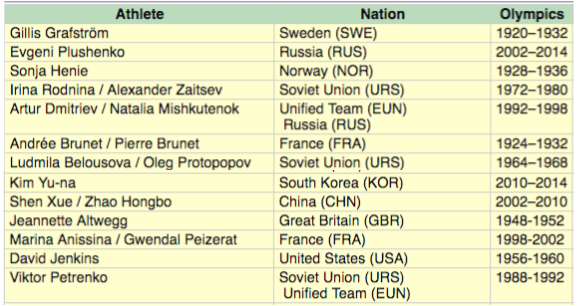
\includegraphics[width=4in]{figures/wikitables_example2.png}
		\caption{Example context from
		\WTQ{}~\citep{pasupat2015compositional}}\label{fig:wikitables_reasoning_example}
	\end{center}
\end{figure}
Consider
Figure~\ref{fig:wikitables_reasoning_example}, which shows part of a table that
provides context for answering some questions in the \WTQ{} dataset. One of the
questions is \textit{Which athlete was from South Korea after the year 2010?}
When we build a semantic parser for this dataset, the model learns to map
questions like these to corresponding logical forms like the following:
\begin{quote}
	\texttt{((reverse athlete) (and (nation south\_korea) (year ((reverse
	date) (>= 2010-mm-dd) ))))}
\end{quote}
If we used a seq2seq model for this task, and simply defined the target
vocabulary to be tokens like \{\texttt{(}, \texttt{)}, \texttt{reverse},
\texttt{athlete}, \texttt{>=}, \ldots\}, then that would let the
model produce any sequence of those tokens, including even those that are
syntactically invalid (say with mismatched parentheses), or semantically invalid
(say with the functions in the logical form taking arguments of incorrect
types). Given enough data, the model could learn to assign lower scores to such
sequences. But the model still has to spend some learning capacity on
distinguishing valid sequences from invalid ones, while we could easily encode
the knowledge required to make that distinction as hard constraints, in the form
of a grammar. In this chapter we show that doing so lets the model learn the
difficult aspects of the semantic parsing more effectively. Using a grammar that
is automatically induced from the types of predicates and entities used in
logical forms, we transform the decoder into a transition based transducer
(i.e., instead of producing tokens like the ones shown above, the decoder
produces transition actions from the grammar that incrementally build the
logical form top down; details in Section~\ref{sec:nnsp_decoder}, and an example
in Figure~\ref{fig:grammar_derivation}.)

\section{Need for Entity Linking}
While building semantic parsers for unrestricted domains like Wikipedia tables
(which is the case with \WTQ{}), one of the most important challenges is to
having to deal with previously unseen entities. This problem gets exacerbated when
the model also learns representations for input tokens, since we will not have
enough training data to learn representations for most of the entities the model
encounters at test time.

To deal with this issue, we first embed a knowledge graph extracted from the
table that provides context to answer a given question, such that entities in
the graph are embedded as a function of their type and neighborhood. Second, we
make the encoded representations of the question context-aware, by augmenting
the input representations of the tokens with a \emph{link embedding}, which is
an expected value of all the entities to which the given token can be softly
linked\footnote{Note that this idea is very similar to the one we used to
obtain ontology grounded token representations in Chapter~\ref{chapter:ontolstm}}.
Third, we include an attention based entity linking module in the decoder, and
score transitions that produce table-specific entities using using this module,
thus effectively side-stepping having to learn representations for them.


We train our model using the Static MML objective. As described in Section~\ref{sec:mml} in
Chapter~\ref{chapter:reasoning_related_work}, the objective
relies on a precomputed set of approximate logical forms that produce the
correct answer, but are not necessarily true translations of the question. We
use Dynamic Programming on Denotations (DPD) followed by pruning based on human
annotations on fictitious tables, as described in~\cite{pasupat2016inferring} to
obtain that set.

We evaluate our parser on \WTQ{}.  This data set has
a broad variety of entities and relations across different tables, along with
complex questions that necessitate long logical forms.  On this data set, our
parser achieves a question answering accuracy of 43.3\% and an ensemble of 5
parsers achieves 45.9\%.  We further perform
several ablation studies that demonstrate the importance of both grammar
constraints and entity linking to achieving high accuracy on this task.

\section{Grammar-Constrained Neural Semantic
Parser}\label{sec:grammar_constrained_model}
\begin{figure}
\centering
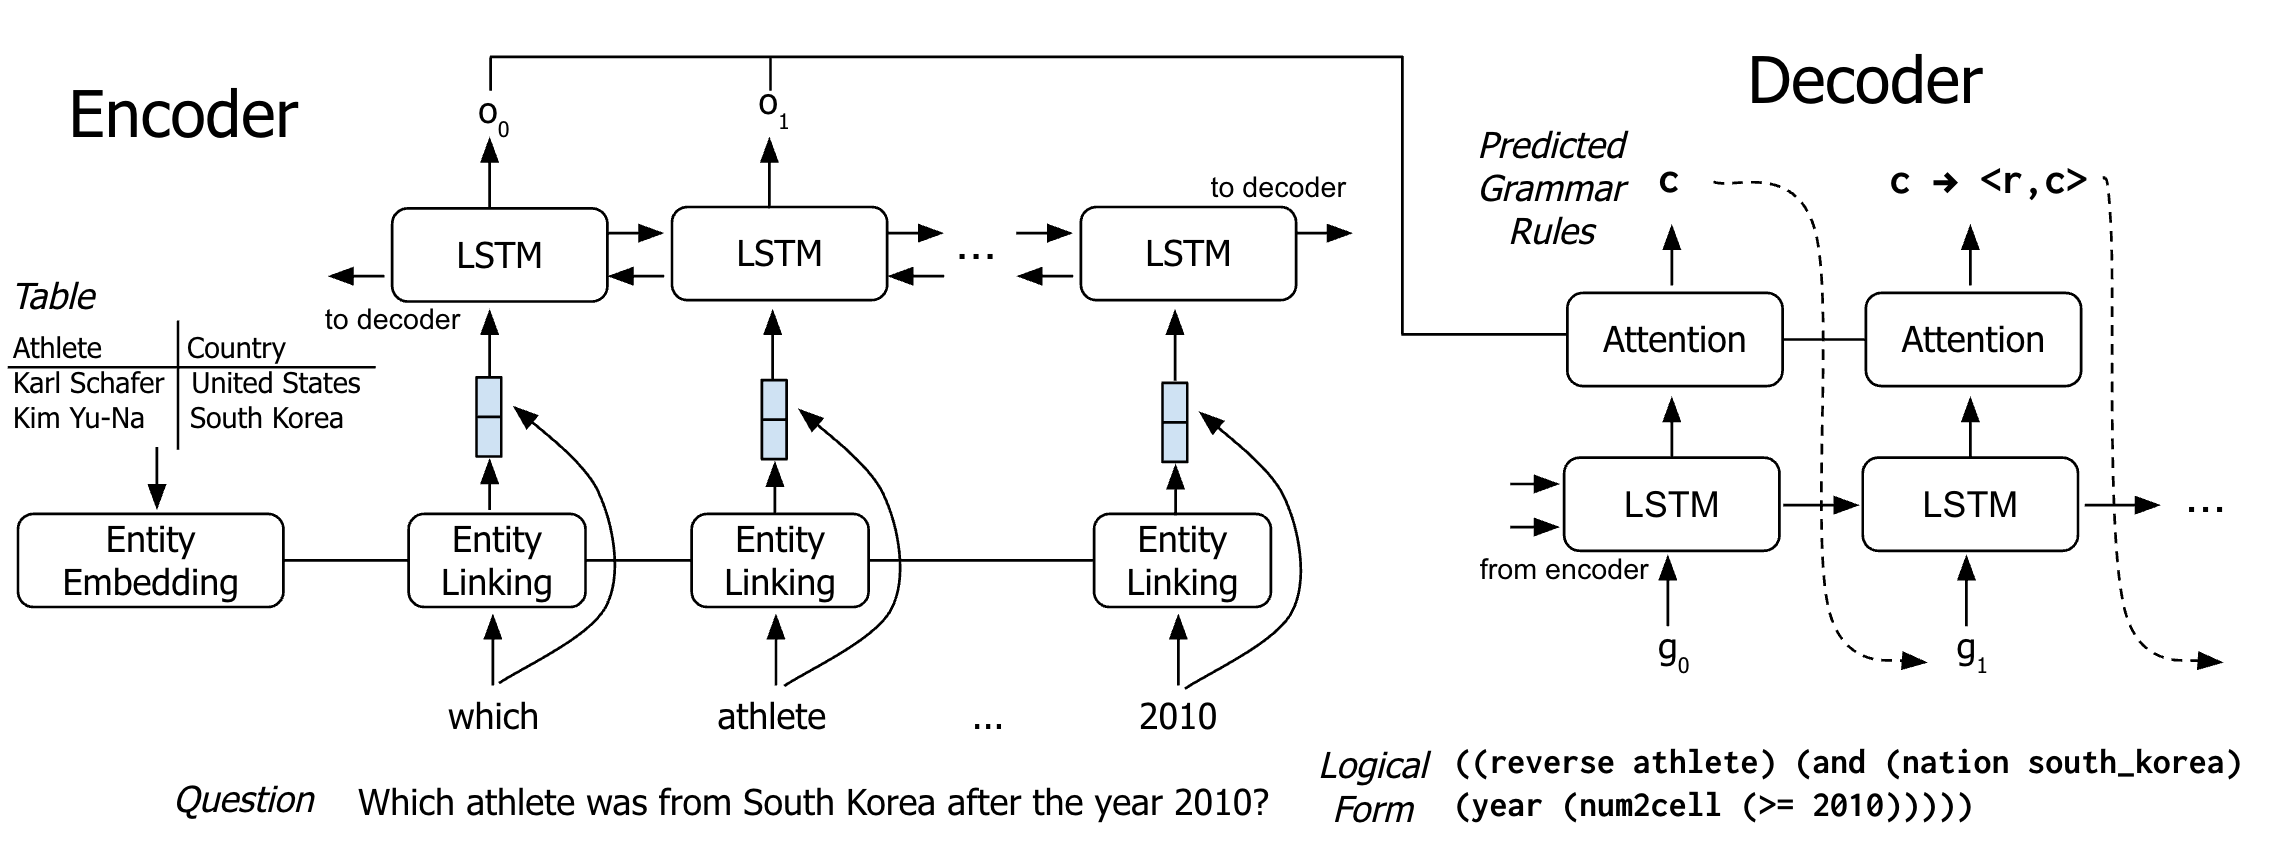
\includegraphics[width=6in]{figures/type_constrained_nnsp.png}
\caption{Overview of our type-constrained neural semantic parsing model}\label{fig:nnsp_model}
\end{figure}

This section describes our semantic parsing model.
The input to our model is a natural language question and a context in which it 
is to be answered.
The model predicts the answer to the question by semantically parsing it to a 
logical form then executing it against the context.

Our model follows an encoder-decoder architecture, using recurrent neural 
networks with Long Short Term Memory (LSTM) cells~\citep{hochreiter1997long}. 
The input question and table entities are first encoded as vectors that are 
then decoded into a logical form (Figure~\ref{fig:nnsp_model}).
We make two significant additions to the standard encoder-decoder architecture.
First, the encoder includes a special entity embedding and linking module that 
produces a \emph{link embedding} for each question token that represents the 
table entities it links to (Section~\ref{sec:nnsp_encoder}).
These link embeddings are concatenated with word embeddings for each question 
token, then encoded with a bidirectional LSTM\@.
Second, the action space of the decoder is defined by a \emph{type-constrained 
grammar} which guarantees that generated logical forms satisfy type constraints 
(Section~\ref{sec:nnsp_decoder}).
The decoder architecture is simply an LSTM with attention that predicts a 
sequence of generation actions within this grammar.

We train the parser using question-answer pairs as supervision, using an 
objective based on enumerating logical forms via dynamic programming on 
denotations \citep{pasupat2016inferring} (Section~\ref{sec:nnsp_training}). This 
objective function makes it possible to train neural models with 
question-answer supervision, which is otherwise difficult for efficiency and 
gradient variance reasons.

\subsection{Encoder}\label{sec:nnsp_encoder}

The encoder network is a standard bidirectional LSTM augmented with an entity 
embedding and linking module.

\paragraph{Notation}
Throughout this section, we denote entities as $e$, and their corresponding 
types as $\tau(e)$. The $i^{\text{th}}$ token in a question is denoted $q_i$. 
We use $v_w$ to denote a learned vector representation (embedding) of word $w$, 
e.g., $v_{q_i}$ denotes the vector representation of the $i$th question token. 
Finally, we denote the set of all entities as $E$, and all entities belonging 
to a type $\tau$ as $E_{\tau}$. The entities $E$ include all of the entities 
from the table, as well as numeric entities detected in the question by NER. 

\paragraph{Entity Embedding}
The encoder first constructs an embedding for each entity in the knowledge 
graph given its type and position in the graph. 
Let $W(e)$ denote the set of words in the name of entity $e$ and $N(e)$ the 
neighbors of entity $e$ in the knowledge graph.
Each entity's embedding $r_e$ is a nonlinear projection of a type vector 
$v_{\tau(e)}$ and a neighbor vector $v_{N(e)}$:
\begin{align}
    v_{N(e)} &= \sum_{e' \in N(e)}\sum_{w \in W(e')}v_w \\
    r_e &= \tanh\big(P_\tau v_{\tau(e)} + P_N v_{N(e)}\big)
\end{align}
The type vector $v_{\tau(e)}$ is a one-hot vector for $\tau(e)$, with dimension 
equal to the number of entity types in the grammar. The neighbor vector 
$v_{N(e)}$ is simply an average of the word vectors in the names of $e$'s 
neighbors. $P_\tau$ and $P_N$ are learned parameter matrices for combining 
these two vectors.

\paragraph{Entity Linking}
This module generates a \emph{link embedding} $l_{i}$ for each question token 
representing the entities it links to.
The first part of this module generates an entity linking score $s(e,i)$ 
for each entity $e$ and token index $i$:

\begin{align}
s(e,i) & = \max_{w \in W(e)} v_w^\intercal v_{q_i} + \psi^\intercal \phi(e,i)
\end{align}

This score has two terms. The first represents similarity in word embedding 
space between the token and entity name, computed as function of the embeddings 
of words in $W(e)$ and the word embedding of the $i$th token, $v_{q_i}$. The 
second represents a linear classifier with parameters $\psi$ on features 
$\phi(e,i)$.
The feature function $\phi$ contains only a few features: exact token match, 
lemma match, edit distance, an NER indicator feature, and a bias feature.
It also includes token and lemma features coming from the neighbors of the node
that originally matches the token. We found that features were an effective way
to address sparsity in the entity name tokens, many of which appear too 
infrequently
to learn embeddings for.

Finally, the entity embeddings and linking scores are combined to produce a 
link embedding for each token.
The scores $s(e,i)$ are then fed into a softmax layer over all entities $e$ of 
the same type, and the link embedding $l_{i}$ is an average of entity vectors 
$r_e$ weighted by the resulting distribution.
We include a null entity, $\varnothing$, in each softmax layer to permit the 
model to identify tokens that do not refer to an entity. The null entity's 
embedding is the all-zero vector and its score $s(\varnothing, \cdot) = 0$.

\begin{align}
%p(e | q_i, \tau(e)) & = \frac{\exp{s(e,q_i)}}{1 + \sum_{e} \exp{s(e,q_i)}} \\
%v_i & = \sum_{\tau} \sum_e v_e p(e | q_i, \tau)
p(e | i, \tau) & = \frac{\exp{s(e,i)}}{\sum_{e'\in E_\tau \cup \{\varnothing\}} 
\exp{s(e',i)}} \\
l_{i} & = \sum_\tau \sum_{e \in E_\tau} r_e p(e | i, \tau)
\end{align}

\paragraph{Bidirectional LSTM}
We concatenate the link embedding $l_i$ and the word embedding $v_{q_i}$ of 
each token in the question, and feed them into a bidirectional LSTM:

\begin{align}
x_i &= \begin{bmatrix} l_{i} \\ v_{q_i} \end{bmatrix} \\
(o^f_i, f_i) &= \text{LSTM}(f_{i-1}, x_i) \\
(o^b_i, b_i) &= \text{LSTM}(b_{i+1}, x_i) \\
o_i &= \begin{bmatrix} o^f_i \\  o^b_i \end{bmatrix}
\end{align}

This process produces an encoded vector representation of each token $o_i$. The 
final LSTM hidden states $f_n$ and $b_{-1}$ are concatenated  and used to 
initialize the decoder.

\subsection{Decoder}\label{sec:nnsp_decoder}

The decoder is an LSTM with attention that selects parsing actions from a 
grammar over well-typed logical forms.

\paragraph{Type-Constrained Grammar} The parser maintains a state at each step 
of decoding that consists of a logical form with typed \emph{holes}.
A hole is a tuple \hole{\tau}{\Gamma} of a type $\tau$ and a \emph{scope} 
$\Gamma$ that contains typed variable bindings, $(x:\alpha) \in \Gamma$.
The scope is used to store and generate the arguments of lambda expressions. 
The grammar consists of a collection of four kinds of production rules on holes:

\begin{enumerate}
    \item \textbf{Application} 
\hole{\tau}{\Gamma}$\rightarrow$\pred{(}\hole{\func{\beta}{\tau}}{\Gamma}~\hole{\beta}{\Gamma}\pred{)}
rewrites a hole of type \type{\tau} by applying a 
function from \type{\beta} to \type{\tau} to an argument of type \type{\beta}. 
We also permit applications with more than one argument.
    \item \textbf{Constant} \hole{\tau}{\Gamma}$\rightarrow$\pred{const} where 
constant \pred{const} has type \type{\tau}. This rule generates both 
context-independent operations such as \pred{argmax} and context-specific 
entities such as\\
\pred{united\_states}.
    \item \textbf{Lambda} \hole{\func{\alpha}{\tau}}{\Gamma}$\rightarrow 
\lambda x$. \hole{\tau}{\Gamma \cup \{(x : \alpha)\}} generates a lambda 
expression where the argument has type \type{\alpha}. $x$ is a fresh variable 
name.
    \item \textbf{Variable} \hole{\tau}{\Gamma}$\rightarrow x$ where $(x : 
\tau) \in \Gamma$. This rule generates a variable bound in a 
previously-generated lambda expression that is currently in scope.
\end{enumerate}

We instantiate each of the four rules above by replacing the type variables 
$\tau, \alpha,\beta$ with concrete types, producing, e.g., $\hole{c}{\Gamma} 
\rightarrow (\hole{\func{r}{c}}{\Gamma}~\hole{r}{\Gamma})$ from the application 
rule.
The set of instantiated rules is automatically derived from a corpus of logical 
forms, which we in turn produce by running dynamic programming on denotations 
(see Section~\ref{sec:nnsp_training}).
Every logical form can be derived in exactly one way using the four kinds of 
rules above; this derivation is combined with the (automatically-assigned) type 
of each of the logical form's subexpressions to instantiate the type variables 
in each rule.
We then filter out constant rules that generate context-specific entities 
(which are 
handled specially by the decoder) to produce a 
context-independent grammar.

\begin{figure}
\centering
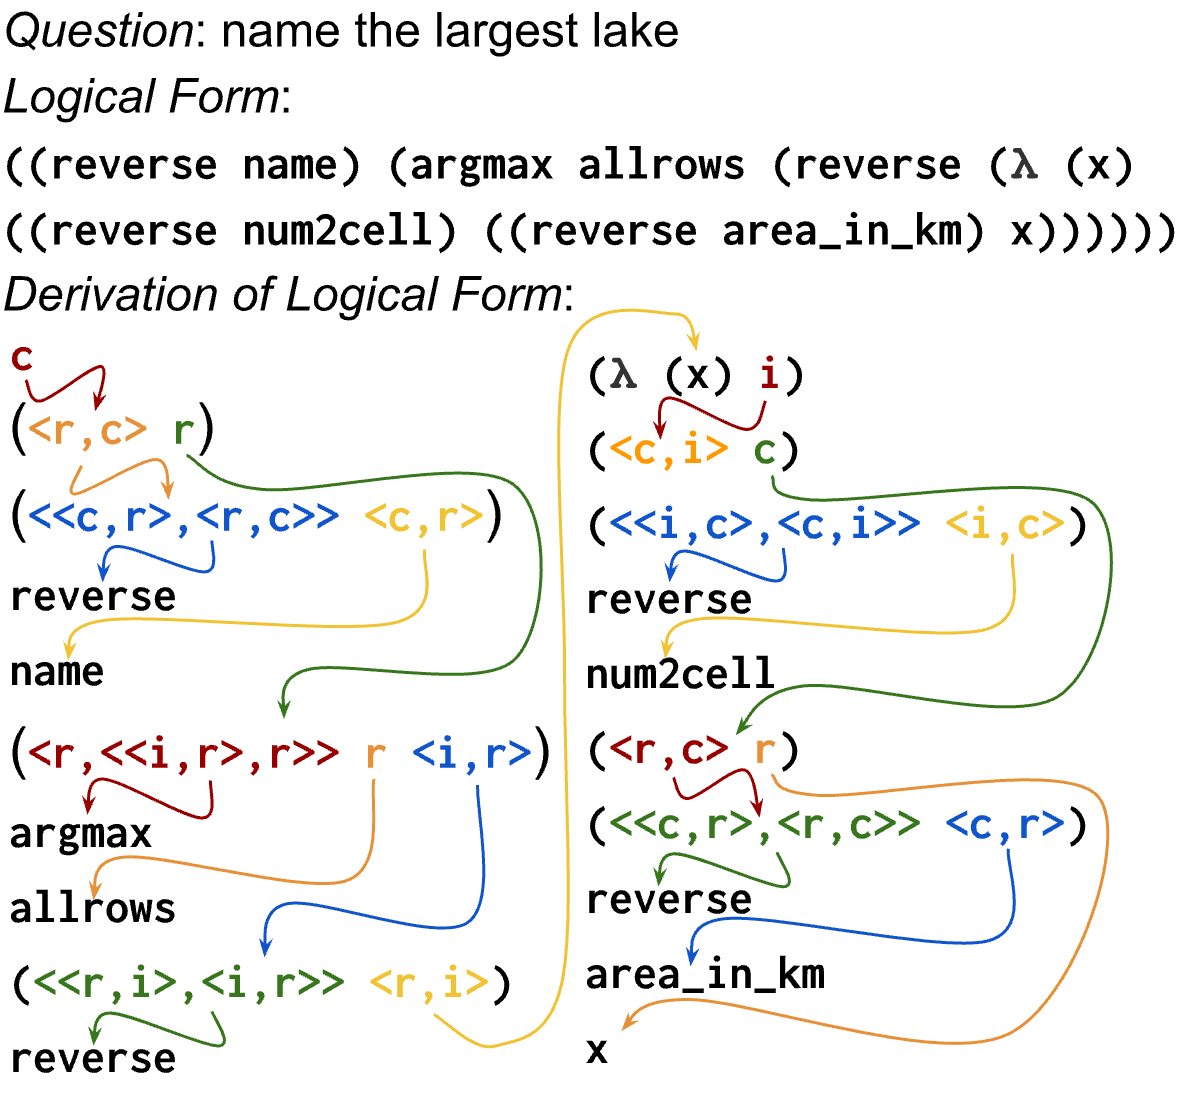
\includegraphics[width=3in]{figures/nnsp_example_derivation.png}
\caption{The derivation of a logical form using the  type-constrained grammar. 
The holes in the left column have 
empty scope, while holes in the right column have scope $\Gamma = \{(x : 
\type{r})\}$}\label{fig:grammar_derivation}
\end{figure}

The first action of the parser is to predict a root type for the logical form, 
and then decoding proceeds according to the production rules above.
Each time step of decoding fills the leftmost hole in the logical form, and 
decoding terminates when no holes remain.
Figure~\ref{fig:grammar_derivation} shows the sequence of decoder actions used 
to generate a logical form.

\paragraph{Network Architecture} The decoder is an LSTM that outputs a 
distribution over grammar actions using an attention mechanism over the encoded 
question tokens. The decoder also uses a copy-like mechanism on the entity 
linking scores to generate entities.
Say that, during the $j$th time step, the current hole has type $\tau$. The 
decoder generates a score for each grammar action whose left-hand side is 
$\tau$ using the following equations:

\begin{align}
 (y_j, h_j) & = \text{LSTM}(h_{j-1}, \begin{bmatrix}g_{j-1} \\ 
o_{j-1}\end{bmatrix}) \label{eq:nnsp_decoder_lstm} \\
 a_j & = \text{softmax}(O W^a y_j) \label{eq:nnsp_decoder_lstm_output}\\
 o_j & = (a_j)^T O  \label{eq:nnsp_decoder_soft_att}\\
 s_j & = W^2_\tau \text{ReLU}( W^1 \begin{bmatrix}y_j \\ o_j \end{bmatrix} + 
b^1) + b^2_\tau \label{eq:nnsp_score_rules}\\
 s_j(e_k) & = \sum_i s(e_k, i) a_{ji} \label{eq:nnsp_score_type}\\
 p_j & = \text{softmax}( \begin{bmatrix} s_j \\ s_j(e_1) \\ s_j(e_2) \\\dots 
\end{bmatrix} ) \label{eq:nnsp_score_action}
\end{align}

The input to the LSTM $g_{j-1}$ is a grammar action embedding for the action 
chosen in previous time step. $g_0$ is a learned parameter vector, and $h_0$ is 
the concatenated hidden states of the encoder LSTMs. The matrix $O$ contains 
the encoded token vectors $o_1, \ldots, ,o_n$ from the encoder. 
\Crefrange{eq:nnsp_decoder_lstm}{eq:nnsp_decoder_soft_att} above perform a 
softmax attention over $O$ using a learned parameter matrix $W^a$. 
Equation~\ref{eq:nnsp_score_rules} generates scores $s$ for the 
context-independent grammar rules applicable to type $\tau$ using a multilayer 
perceptron with weights $W^1$,$b^1$,$W^2_\tau$,$b^2_\tau$. 
Equation~\ref{eq:nnsp_score_type} generates a score for each entity $e$ with 
type $\tau$ by averaging the entity linking scores with the current attention 
$a_j$. Finally, the context-independent and -dependent scores are concatenated 
and softmaxed to produce a probability distribution $p_j$ over grammar actions 
in Equation~\ref{eq:nnsp_score_action}. If a context-independent action is 
chosen, $g_{j}$ is a learned parameter vector for that action. Otherwise $g_{j} 
= g^\tau$, which is a learned parameter representing the selection of an entity 
with type $\tau$.


\section{Experiments with \WTQ{}}
We now describe an application of our framework to \WTQ{}, 
a challenging dataset for question
answering against semi-structured Wikipedia
tables~\citep{pasupat2015compositional}. An example question from this dataset
is shown in Figure~\ref{fig:wikitables_reasoning_example}.

\subsection{Context and Logical Form Representation}\label{sec:preliminaries}

We follow~\citep{pasupat2015compositional} in using the same table structure 
representation 
and $\lambda$-DCS language for expressing logical forms.
In this representation, tables are expressed as knowledge graphs over 6 types 
of 
entities: cells, cell parts, rows, columns, numbers and dates.
Each entity also has a name, which is typically a string value in the table.
Our parser uses both the entity names and the knowledge graph structure to 
construct embeddings for each entity. Specifically, the neighbors of a column 
are the cells it
contains, and the neighbors of a cell are the columns it belongs to.

The logical form language consists of a collection of named sets and entities, 
along with operators on them.
The named sets are used to select table cells, e.g., \pred{united\_states} is 
the set of cells that contain the text ``united states''.
The operators include functions from sets to sets, e.g., the \pred{next} 
operator maps a row to the next row.
Columns are treated as functions from cells to their rows, e.g., \pred{(country 
united\_states)} generates the rows whose \pred{country} column contains 
``united states''. 
Other operators include reversing relations (e.g., in order to map rows to 
cells 
in a certain column), relations that interpret cells as numbers and dates, and 
set and arithmetic operations. 
The language also includes aggregation and quantification operations such as 
\pred{count} and \pred{argmax}, along with $\lambda$ abstractions that can be 
used to join binary relations.

Our parser also assigns a type to every $\lambda$-DCS expression, which is used 
to enforce type constraints on generated logical forms.
The base types are cells \type{c}, parts \type{p}, rows \type{r}, numbers 
\type{i}, and dates \type{d}.
Columns such as \pred{country} have the functional type \func{c}{r}, 
representing functions from cells \type{c} to rows \type{r}.
Other operations have more complex functional types, e.g., \pred{reverse} has 
type
\func{\func{c}{r}}{\func{r}{c}}, which enables us to write \pred{(reverse 
country)}.\footnote{Technically, \pred{reverse} has the parametric polymorphic 
type \func{\func{\alpha}{\beta}}{\func{\beta}{\alpha}}, where \type{\alpha} and 
\type{\beta} are \emph{type variables} that can be any type. This type allows 
\pred{reverse} to reverse any function. However, this is a detail that can 
largely be ignored. We only use parametric polymorphism when typing logical 
forms to generate the type-constrained grammar; the grammar itself does not 
have 
type variables, but rather a fixed number of concrete instances -- such as 
\func{\func{c}{r}}{\func{r}{c}} -- of the above polymorphic type.}
The parser assigns every $\lambda$-DCS constant a type, then applies standard 
programming language type inference algorithms~\citep{Pierce2002TypesAP} to 
automatically assign types to larger expressions.

\subsection{Training with Offline Search}
\label{sec:nnsp_training}
Our parser is trained from question-answer pairs, treating logical forms as a 
latent variable. We use a new loglikelihood objective function for this process 
that first automatically enumerates a set of correct logical forms for each 
example, then trains on these logical forms. This objective simplifies the 
search problem during training and is well-suited to training our neural model.

The training data consists of a collection of $n$ question-answer-table 
triples, 
$\{(q^i, a^i, T^i)\}_{i=1}^n$. We first run dynamic programming on
denotations~\citep{pasupat2016inferring} on each table $T^i$ and answer $a^i$ to generate a 
set of 
logical forms $\ell \in \mathcal{L}^i$ that execute to the correct answer.

\paragraph{Dynamic programming on denotations}
DPD is an automatic procedure for enumerating logical forms that execute to produce a particular value; it leverages the 
observation that there are fewer denotations than logical forms to enumerate 
this set relatively efficiently. It is a kind of chart parsing algorithm where
partial parses are grouped together in cells by their output category, size, and
the denotation. This is an improvement over the previous work by~\cite{pasupat2015compositional},
where the logical forms were grouped based on only the output category and size.
Given this chart, DPD performs two forward passes, In the first pass, the algorithm
finds all the cells that lead to the correct denotation. In the second pass, all the
rule combinations which lead to the cell corresponding to the correct denotation
are listed, and logical forms are generated from those cells, using only the rule combinations
that are known to lead to the final cells.

Followed by this
process,~\cite{pasupat2016inferring} also prune the resulting logical forms
to remove spurious ones. Recall that as described in
Section~\ref{sec:weak_supervision}, spurious logical forms are those that yield
the correct answer, but only coincidentally so, since they are not true
translations of the original questions. The insight behind the pruning process
is that a correct logical form will produce the correct logical form even if the
contents of the table are are shuffled around, whereas a spurious one may not
(see the original paper for more details). We use the filtered set of logical
forms, and train the model with the following Static MML objective: 

\begin{align}
    \mathcal{O}(\theta) & = \sum_{i=1}^n \log \sum_{\ell \in \mathcal{L}^i} 
P(\ell | q^i, T^i; \theta )
\end{align}

We optimize this objective function using stochastic gradient descent.
If $|\mathcal{L}^i|$ is small, e.g., 5-10, the gradient of the $i$th example 
can 
be computed exactly by simply replicating the parser's network architecture 
$|\mathcal{L}^i|$ times, once per logical form.
(Note that this takes advantage of the property that each logical form has a 
unique derivation in the decoder's grammar.)
However, $|\mathcal{L}^i|$ often contains many thousands of logical forms, 
which 
makes the above computation infeasible. We address this problem by truncating 
$\mathcal{L}^i$ to the $m=100$ shortest logical forms, then using a beam search 
with a beam of $k=5$ to approximate the sum.

We briefly contrast this objective function with two other commonly-used 
approaches. The first approach is commonly used in prior semantic parsing work 
with loglinear models~\citep{Liang2011LearningDC,pasupat2015compositional} and 
uses a similar 
loglikelihood objective. The gradient computation for this objective requires 
running a wide beam search, generating, e.g., 300 logical forms, executing each 
one to identify which are correct, then backpropagating through a term for 
each. 
This process would be very expensive with a neural model due to the cost of 
each 
backpropagation pass. Another approach is to train the network with
REINFORCE~\citep{williams1992simple}, which essentially samples a logical form instead of 
using 
beam search. This approach is known to be difficult to apply when the space of 
latent variables is large and the reward signal sparse, as it is in semantic 
parsing. Our objective improves on these by precomputing correct logical forms 
in order 
to avoid searching for them during the gradient computation.

\subsection{Experimental Setup}
We used the standard train/test splits of \textsc{WikiTableQuestions}.
The training set consists of 14,152 examples and the test set consists of 4,344 
examples.
The training set comes divided into 5 cross-validation folds for development 
using an 80/20 split.
All data sets are constructed so that the development and test tables are not 
present in the training set.
We report question answering accuracy measured using the official evaluation 
script, which performs some simple normalization of numbers, dates, and strings 
before comparing predictions and answers.
When generating answers from a model's predictions, we skip logical forms that 
do not execute (which may occur for some baseline models) or answer with the 
empty string (which is never correct).
All reported accuracy numbers are an average of 5 parsers, each trained on one 
training fold, using the respective development set to perform early stopping.

We trained our parser with 20 epochs of stochastic gradient descent. We used 
$200$-dimensional word embeddings for the question and entity tokens, mapping 
all tokens that occurred $<3$ times in the training questions to \texttt{UNK}. 
(We tried using a larger vocabulary that included frequent tokens in tables, 
but this caused the parser to seriously overfit the training examples.) The 
hidden and output dimensions of the forward/backward encoder LSTMs were set to 
$100$, such that the concatenated representations were also $200$-dimensional. 
The decoder LSTM uses $100$-dimensional action embeddings and has a 
$200$-dimensional hidden state and output. The action selection MLP has a 
hidden layer dimension of $100$. We used a dropout probability of $0.5$ on the 
output of both the encoder and decoder LSTMs, as well as on the hidden layer of 
the action selection MLP\@. At test time, we decode with a beam size of 10.

\subsection{Results}
Table~\ref{tab:nnsp_wikitables_results} compares the accuracy of our semantic parser 
to prior work on \textsc{WikiTableQuestions}.
We distinguish between single models and ensembles, as we expect ensembling to 
improve accuracy, but not all prior work has used it.
Prior work on this data set includes a loglinear semantic
parser~\citep{pasupat2015compositional}, that same parser with a neural,
paraphrase-based
reranker~\citep{haug2017neural}, and a neural programmer that answers questions by predicting a 
sequence of table operations~\citep{Neelakantan2016LearningAN}.  
We find that our parser outperforms the best prior result on this data set by 
4.6\%, despite that prior result using a 15-model ensemble.
An ensemble of 5 parsers, one per training fold, improves accuracy by an 
additional 2.6\% for a total improvement of 7.2\%.
\begin{table}
    \centering
    \begin{tabular}{lccc}
	\toprule
        \textbf{Model} & \textbf{Ensemble Size} & \textbf{Dev.} & \textbf{Test} \\
        \midrule 
        \cite{Neelakantan2016LearningAN} & 1 & 34.1 & 34.2 \\
        \cite{haug2017neural} & 1 & - & 34.8 \\
        \cite{pasupat2015compositional} & 1 & 37.0 & 37.1 \\
        \cite{Neelakantan2016LearningAN} & 15 & 37.5 & 37.7 \\
        \cite{haug2017neural} & 15 & - & 38.7 \\
        \midrule
        Our Parser & 1 & 42.7 & 43.3 \\
        Our Parser & 5 & - & \textbf{45.9} \\
        \bottomrule
    \end{tabular}
    \caption{Development and test set accuracy of our semantic parser compared
	to prior work on \textsc{WikiTableQuestions}}\label{tab:nnsp_wikitables_results}
\end{table}

This ensemble was constructed by averaging the logical form probabilities of
parsers trained on each of the 5 cross-validation folds.  Note that this
ensemble is trained on the entire training set --- the development data from one
fold is training data for the others --- so we therefore cannot report its
development accuracy.  We investigate the sources of this accuracy improvement
in the remainder of this section via ablation experiments.

\subsection{Type Constraints}

Our second experiment measures the importance of type constraints on the decoder
by comparing it to sequence-to-sequence (seq2seq) and sequence-to-tree
(seq2tree) models.  The seq2seq model generates the logical form a token at a
time, e.g., $[ (, (,$\pred{reverse}$,\ldots]$, and has been used in several
recent neural semantic parsers~\citep{jia2016,dong2016}.  The seq2tree model
improves on the seq2seq model by including an action for generating matched
parentheses, then recursively generating the subtree within~\citep{dong2016}.
These baseline models use the same network architecture (including entity
embedding and linking) and training regime as our parser, but assign every
constant the same type and have a different grammar in the decoder.  These
models were implemented by preprocessing logical forms and applying a different
type system.

Table~\ref{tab:typing_results} compares the accuracy of our parser to both the
seq2seq and seq2tree baselines.  Both of these models perform considerably worse
than our parser, demonstrating the importance of type constraints during
decoding.  Interestingly, we found that both baselines typically generate
well-formed logical forms: only 7.4\% of seq2seq and 6.6\% of seq2tree's
predicted logical forms failed to execute.  Type constraints prevent these
errors from occurring in our parser, though the relatively small number of such
errors does not does not seem to fully explain the 9\% accuracy improvement.  We
hypothesize that the additional improvement occurs because type constraints also
increase the effective capacity of the model, as both the seq2seq and seq2tree
models must use some of their capacity to learn the type constraints on logical
forms.

\begin{table}[]
	\centering
	\begin{tabular}{lc} \toprule
	\textbf{Model} & \textbf{Dev. Accuracy} \\ \midrule
	seq2seq & 31.3 \\
	seq2tree & 31.6 \\
	Our Parser & 42.7 \\ \bottomrule
	\end{tabular}
	\caption{Development accuracy of our semantic parser compared to
	sequence-to-sequence and sequence-to-tree models.}\label{tab:typing_results}
\end{table}

\subsection{Entity Embedding and Linking}
Our next experiment measures the contribution of the entity embedding and
linking module. We trained several ablated versions of our parser, removing both
the embedding similarity and featurized classifier from the entity linking
module. Table~\ref{tab:el_results} shows the accuracy of the resulting models.
The results demonstrate that the entity linking features are important,
particularly the more complex features beyond simple token matching. In our
experience, the ``related column'' features are especially important for this
data set, as columns that appear in the logical form are often not mentioned in
the text, but rather implied by a mention of a cell from the column. Embedding
similarity alone is not very effective, but it does improve accuracy when
combined with the featurized classifier. We found that word embeddings enabled
the parser to overfit, which may be due to the relatively small size of the
training set, or because we did not use pretrained embeddings. Incorporating
pretrained embeddings is an area for future work.

We also examined the effect of the entity embeddings computed using each
entity's knowledge graph context by replacing them with one-hot vectors for the
entity's type. The accuracy of this parser dropped from 42.7\% to 41.8\%,
demonstrating that the knowledge graph embeddings help.

\begin{table}
	\centering
	\begin{tabular}{lc} \toprule
	\textbf{Model} & \textbf{Dev. Accuracy} \\ \midrule 
	Full model & 42.7 \\ 
        \quad w/o entity embeddings & 41.8 \\
	\quad token features, no similarity & 28.1 \\
	\quad all features, no similarity & 37.8 \\
	\quad similarity only, no features & 27.5 \\ \bottomrule
	\end{tabular}
	\caption{Development accuracy of ablated parser variants
	trained without parts of the entity linking module.}\label{tab:el_results}
\end{table}

\subsection{DPD Training}
\label{sec:experiments_dpd}
Our final experiment examines the impact on accuracy of varying the number of
logical forms $m$ used when training with dynamic programming on denotations.
Table~\ref{tab:dpd_results} shows the development accuracy of several parsers
trained with varying $m$. These results demonstrate that using more logical
forms generally leads to higher accuracy.

\begin{table}
	\centering
	\begin{tabular}{lccccc} \toprule
	\# of logical forms & 1 & 5 & 10 & 50 & 100 \\
	Dev. Accuracy & 39.7 & 41.9 & 41.6 & 43.1 & 42.7 \\ \bottomrule
	\end{tabular}
	\caption{Development accuracy of our semantic parser when trained with
	varying numbers of logical forms produced by dynamic programming on
	denotations.}\label{tab:dpd_results}
\end{table}

\subsection{Error Analysis}

To better understand the mistakes made by our system, we analyzed a randomly
selected set of 100 questions that were answered incorrectly. We identified
three major classes of error:

\paragraph{Parser errors (41\%):} These are examples where a correct logical
form is available, but the parser does not select it. A large number of these
errors (15\%) occur on questions that require selecting an answer from a given
list of options, as in \textit{Who had more silvers, Colombia or The Bahamas?}
In such cases, the type of the predicted answer is often wrong. Another common
subclass is entity linking errors due to missing background knowledge (13\%),
e.g., understanding that \textit{largest} implicitly refers to the \textit{Area}
column.

\paragraph{Representation failures (25\%):} The knowledge graph representation
makes certain assumptions about the table structure and cell values which are
sometimes wrong. One common problem is that the graph lacks some cell parts
necessary to answer the question (15\%). For example, answering a question
asking for a state may require splitting cell values in the \textit{Location}
column into city and state names. Another common problem is unusual table
structures (10\%), such as a table listing the number of Olympic medals won by
each country that has a final row for the totals. These structures often cause
quantifiers such as \pred{argmax} to select the wrong row.

\paragraph{Unsupported operations (11\%):} These are examples where the logical
form language lacks a necessary function. Examples of missing functions are
finding consecutive sets of values, computing percentages and performing string
operations on cell values.

\section{Conclusion}
We introduced in this chapter, two ways to incorporate contextual knowledge into
building neural semantic parsers: grammar constrained
decoding, and context linking. As evidenced by the fact that our
grammar-constrained model out performs seq2seq and seq2tree models trained on
the same data, the constraints provide a useful inductive bias. Moreover, that
the most of the logical forms produced by trained seq2seq and seq2tree models
are also executable, shows that grammar constraints free our model from having
to distinguish valid logical forms from invalid ones, and instead let it learn
deeper semantics. Our joint entity embedding and linking module provides an
effective way to sidestep the issue of having to learn representations for
previously unseen entities.

While our model is weakly supervised, it still assumes a good set of
offline searched logical forms, and we relied on the output from DPD, pruned
using human annotations. In Chapter~\ref{chapter:nlvr}, we further relax this
assumption, and in doing so leverage more contextual knowledge.
